\section{Bilayer graphene}
\label{sec:bilayer}
In the tight-binding description of bilayer graphene, we take into account $2p_z$ orbitals on the four atomic sites in the unit cell, labelled as $j = A_1, B_1, A_2, B_2$. Then, the transfer integral matrix of bilayer graphene is a $4\times 4$  matrix given by \cite{McCann_2013}

\begin{equation}
    H(\vect k)=
    \begin{bmatrix}
        E_{A_1} & -\gamma_0 F(\vect k) & \gamma_4 F(\vect k) & -\gamma_3 F(\vect k)\\
        -\gamma_0 F(\vect k) & E_{B_1} & -\gamma_1 & \gamma_4 F(\vect k)\\
        \gamma_4 F(\vect k) & \gamma_1 & E_{A_2} & -\gamma_0 F(\vect k)\\
        -\gamma_3 F(\vect k)& \gamma_4 F(\vect k)& -\gamma_0 F(\vect k) & E_{B_2}
    \end{bmatrix}\,,
\end{equation}

% 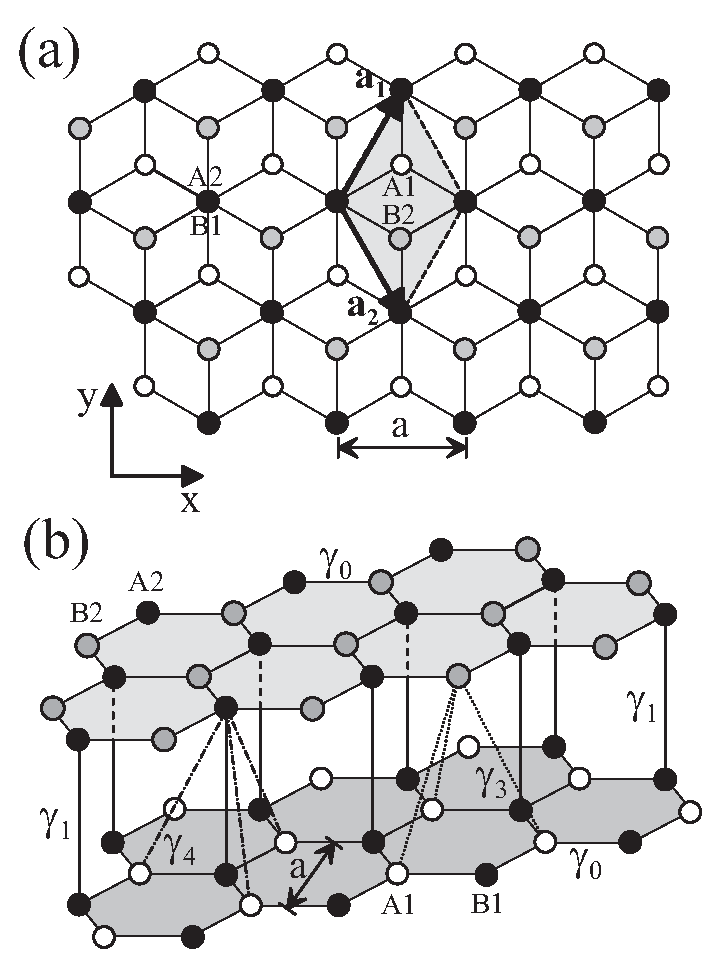
\includegraphics[width=\linewidth]{Immagini/graphene/bilayerlattice.eps}
% \caption{difference between the gapless and the gapped Dirac dispersion relation}
% \label{fig:bilayer-lattice}

\begin{table}[ht]
    \begin{minipage}[b]{0.56\linewidth}
    \centering
    \begin{tabular}{ l l r }
        \hline
        Parameter & Value [eV] \\ 
        \hline \hline
        $\gamma_0$ & $3.16\pm0.03$ \\
        $\gamma_1$ & $0.381\pm 0.003$ \\
        $\gamma_3$ & $0.38\pm 0.06$ \\
        $\gamma_4$ & $0.14\pm 0.03$ \\
        \hline
       \end{tabular}
        \caption{Values in eV of $\gamma_i$ \cite{kuzmenko2009determination}}
        \label{table:valuetable}
    \end{minipage}\hfill
    \begin{minipage}[b]{0.4\linewidth}
    \centering
    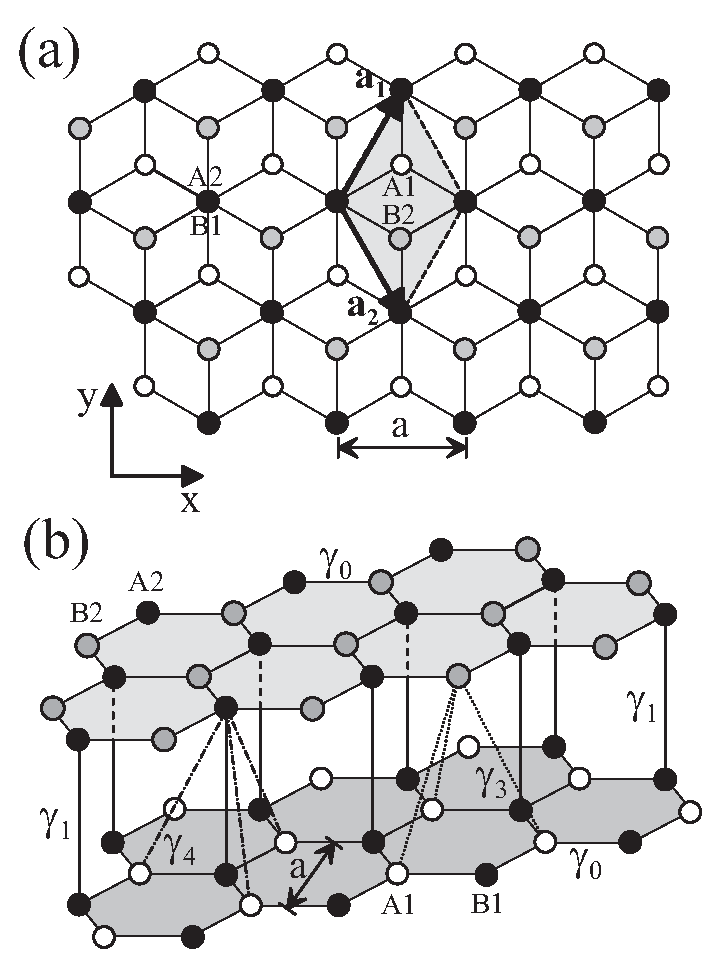
\includegraphics[width=\linewidth]{Immagini/graphene/bilayerlattice.eps}
    \captionof{figure}{Schematic representation of the bilayer graphene structure. Image taken from \cite{McCann_2013}}
    \label{fig:bilayer-lattice}
    \end{minipage}
\end{table}

where the tight-binding parameters are defined as 
\begin{equation}
    \begin{split}
        \gamma_0=&-\braket{A_1|H}{B_1}=-\braket{A_2|H}{B_2}\,; \\
        \gamma_1=&\braket{A_2|H}{B_1} \,; \\
        \gamma_3=&-\braket{A_1|H}{B_2} \,; \\
        \gamma_4=& \braket{A_1|H}{A_2}=\braket{B_1|H}{B_2}\,. \\
    \end{split}
\end{equation}
The upper-right and lower-left square $2\times 2$ blocks of $H$ describe inter-layer coupling. Parameter $\gamma_1$ describes coupling between pairs of orbitals on sites that are directly above each other $B_1$ and $A_2$ (also called dimer sites): since this is a vertical coupling, the corresponding terms in $H$ do not contain $F(\vect k)$ which describes in-plane hopping. The other $\gamma$ factors do have an in plane component, which causes the $F(\vect k)$ term to show up.\\
The overlap matrix $S$ form equation $\ref{eq:overlap}$ becomes in the bilayer case
\begin{equation}
    S=
    \begin{bmatrix}
        1 & s_0 F(\vect k) & 0&0\\
        s_0 F(\vect k)  &1&s_1&0\\
        0&s_1&1&s_0 F(\vect k)\\
        0&0&s_0 F(\vect k) &1
    \end{bmatrix}\,.
\end{equation}
Here we only include two parameters: $s_0 = \braket{A_1}{B_1} = \braket{A_2}{B_2}$ describing non-orthogonality of intra-layer nearest-neighbours and $s_1= \braket{A_2}{B_1}$ describing non-orthogonality of orbitals on dimer sites A1 and B2. In principle, it is possible to introduce additional parameters analogous to $\gamma_3,\gamma_4$, etc., but generally they will be small and irrelevant, infact in the bilayer case it is common practice to neglect completely the overlap matrix if we are dealing with. The resulting energy bands are plotted in figure \ref{fig:dispersion-bilayer}

\begin{figure}[h]
    \makebox[\textwidth][c]{
        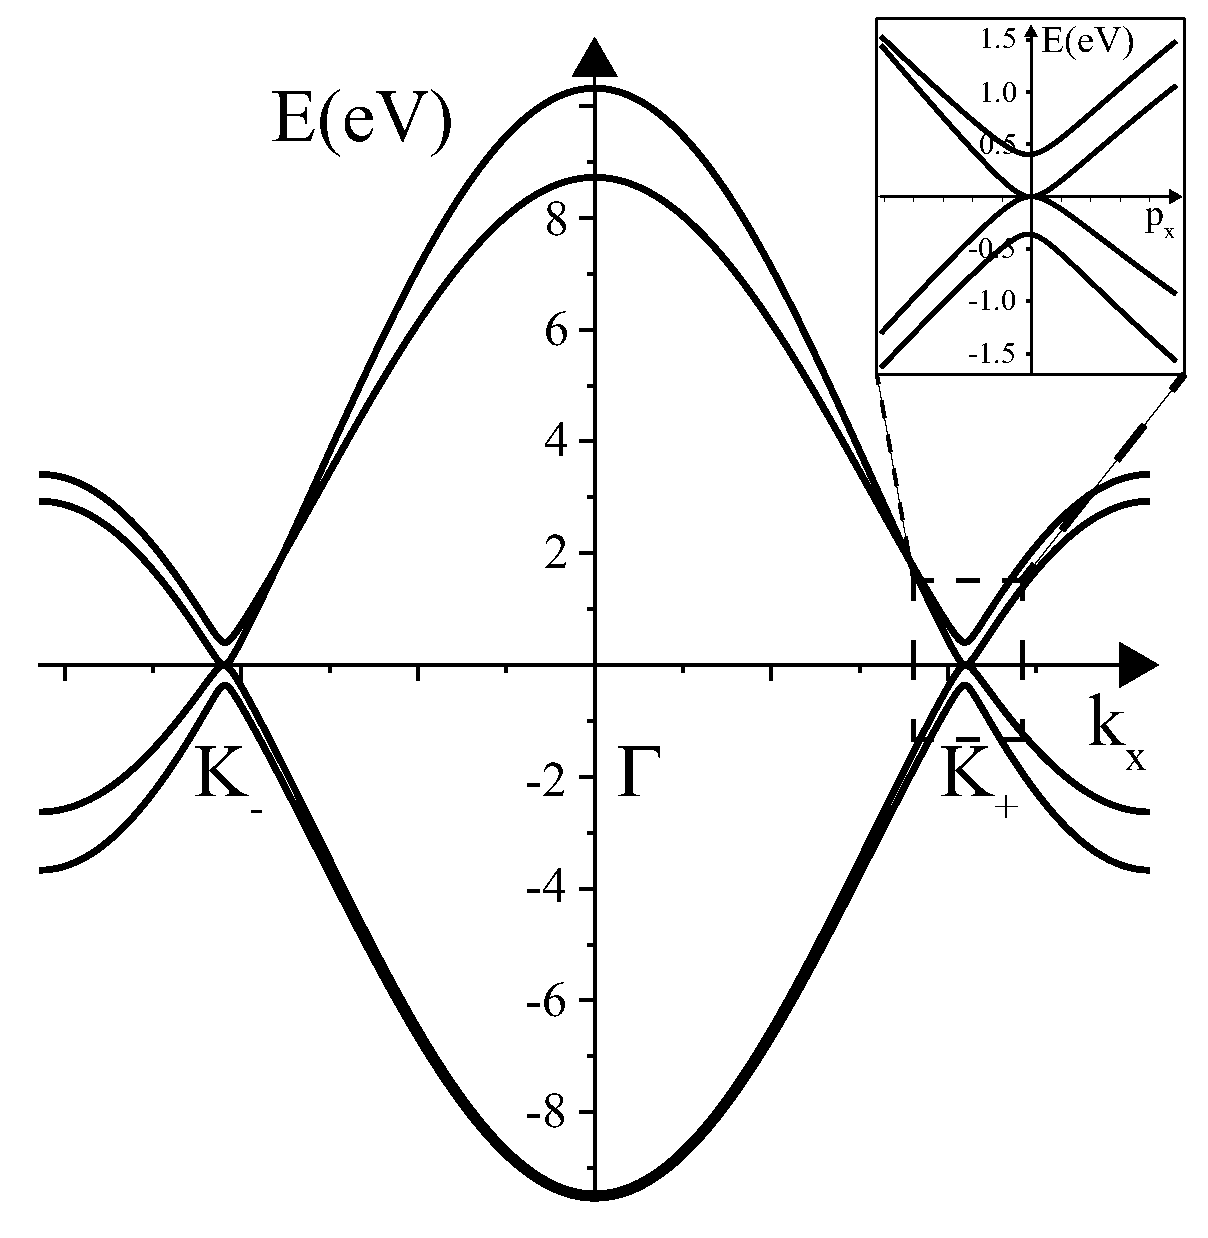
\includegraphics[width=.7\linewidth]{Immagini/graphene/bilayer-bands.eps}
        }%
    \caption{Here are plotted the $p_z$ orbitals along the $k_x$ axis in the reciprocal space intersecting the corners $K_0$ and $K_1$ and the center $\Gamma$ of the Brillouin zone. Notice how now we have four bands, this because we have four atoms in the fundamental cell, two for each layer. Image taken from \cite{McCann_2013}}
    \label{fig:dispersion-bilayer}
\end{figure}
To describe the properties of the electrons near the $K$ we just have to approximate $F(\vect k)$ just like we did in equation \ref{eq:F(k)-approx}. This results in a Hamiltonian that is the generalization of the one we had in equation \ref{eq:gapped-dirac}

\begin{equation}
    H_{\vect K_0}=
    \begin{bmatrix}
        E_{A_1} & v_F\pi^\dag & -v_4\pi^\dag & v_3\pi\\
        v_F\pi& E_{B_1} & \gamma_1 & -v_4\pi^\dag\\
        -v_4\pi & \gamma_1 & E_{A_2} & v_F\pi^\dag\\
        v_3\pi^\dag & -v_4\pi & v_F\pi & E_{B_2}
    \end{bmatrix}\,.
\end{equation}
Where $\pi= \hbar (\tau_zk_x+ik_y),\pi^\dag=\hbar (\tau_zk_x-ik_y)$, and the velocities $v_{3,4}=a\gamma_{3,4}/\hbar$ are effective fermi velocities that come from the coupling $\gamma_3$ and $\gamma_4$






\subsection*{Effective two-band Hamiltonian at low energy}
Most of the properties we are interested in graphene are about the electronic properties near the Dirac points. \\
First we consider the energy eigenvalue equation considering separate blocks in the Hamiltonina corresponding to low-energy $\vect \theta=(\psi_{A1},\psi_{B2})$ and dimer $\vect \chi= (\psi_{A_2},\psi_{B_1})$

\begin{equation}
\begin{bmatrix}
    h_\theta & u\\
    u^\dag & h_\chi
\end{bmatrix}=
\begin{bmatrix}
    \vect \theta\\
    \vect \chi
\end{bmatrix}=
E\begin{bmatrix}
    \vect \theta\\
    \vect \chi
\end{bmatrix}\,.
\label{eq:double-layer-ham-reduced1}
\end{equation}
The second row of \ref{eq:double-layer-ham-reduced1} allows the dimer components to be expressed in terms of the low energy ones.
\begin{equation}
    \vect \chi=(E-h_\chi)^{-1}u^\dag\vect \theta\,,
    \label{eq:chi-as-theta}
\end{equation} 
substituting this into equation \ref{eq:double-layer-ham-reduced1} gives us an effective eigenvalue equation depending on low the low energy components 

\begin{equation}
[h_\theta + u(E-h_\chi)^{-1}u^\dag]\vect \theta=E\vect \theta\,.
\end{equation}
Note that this is not anymore a simple eigenvector problem because the eigenvalue $E$ is a parameter of the matrix we wish to diagonalize, making an approximation it is possible to write the equation above, up to linear terms of the energy like so:
\begin{equation}
    [h_\theta + uh_\chi^{-1}u^\dag]\vect \theta\approx ES\vect \theta\,,
\end{equation}
where $S=1+uh_{\chi}^{-2}u^\dag$ and the second equation is accurate up to a linear term in $E$. We now define $\vect \Phi=S^{1/2}\vect \theta$ and substitute it in the equation above
\begin{equation}
    S^{-1/2}[h_\theta + uh_\chi^{-1}u^\dag]S^{-1/2}\vect \Phi=E\vect \Phi\,.
    \label{eq:double-layer-ham-reduced2}
\end{equation}
With this we can define the effective $2\times 2$ Hamiltonian, find its eigenvectors $\vect \phi$, and then mutliply it by $S^{-1/2}$ to get $\vect \theta=S^{-1/2}\vect\Phi$, and then use equation \ref{eq:chi-as-theta} to get the $\vect \chi$ component.
Remember however that since we have a $2\times 2$ matrix we are going to get two eigenvalues instead of $4$ of the original Hamiltonian if equation \ref{eq:double-layer-ham-reduced1}. These two energies are going to be the ones that touch the Fermi level (figure \ref{fig:dispersion-bilayer}), and $k_bT\ll \Delta E$ higher energy states can be ignored  (here $\Delta E$ is the gap of the high energy states)\\
The effective Hamiltonian is \cite{mccann2006landau,mucha2010electron}
\begin{equation}
\begin{split}
    H=&H_2+h_w+h_4+h_\Delta+h_U+h_{AB}\,,\\
    H_2=&-\frac1 {2m}\begin{bmatrix}
        0 & (\pi^\dag)^2\\
        \pi^2 &0\\
    \end{bmatrix}\,,
\end{split}
\label{eq:bilayer_ham}
\end{equation}
where $H_2$ can is the dominant term and describes massive electrons, and it may be written like so $H_2=-(1/2m)[\sigma_x(p_x^2-p_y^2)+2\tau_z\sigma_yp_xp_y]$. And it dominates at low energies, the other terms may be considered as perturbations of it. the term $h_w$ represents a triangular distortion of the Fermi circle around the $\vect K$. the terms $h_U$ and $h_{AB}$ produce a band gap while $h_4$ and $h_\Delta$ introduce electron-hole asymmetry.
The solutions of $H_0$ are massive chiral electrons with parabolic dispersion $E=\pm p^2/2m,\,\,m=\gamma_1/2v^2$ and the corresponding wavefunctions are
\begin{equation}
    \ket{\pm,\vect k}=
    \frac 1{\sqrt 2}
    \begin{bmatrix}
        1\\
        \mp e^{2i\tau_z\phi}
    \end{bmatrix}
    e^{i\vect k\cdot \vect r}\,,
    \label{eq:bilayer_eigenstates}
\end{equation}
where the wavefunction components describe the electronic amplitudes pf the $A1$ and $B2$ sites.